\begin{abstract}
Lorem ipsum dolor sit amet, consectetur adipiscing elit. Nam eu dolor pretium,
egestas mauris sed, dapibus quam. Duis hendrerit mollis nunc a consequat. Nulla
et sem consectetur, interdum velit eget, aliquam ipsum. Praesent sagittis
tortor diam, sed ultrices magna ullamcorper vitae. Proin vitae orci augue.
Morbi dictum ligula gravida sem malesuada facilisis. Mauris nibh metus, cursus
eget imperdiet vitae, pretium at lorem. Praesent nisi mauris, pretium ut risus
fermentum, egestas tincidunt nibh. Mauris nulla orci, consequat eu pharetra
non, mattis ut urna. Mauris facilisis orci eros. Nam mattis non magna iaculis
consectetur. Morbi sodales dolor vitae felis sagittis, eget faucibus turpis
convallis. Nullam malesuada, mauris et ultricies rutrum, odio nulla gravida
nunc, ac volutpat eros lectus eget lacus. Integer venenatis velit vel justo
pellentesque, quis molestie sem vestibulum.
\end{abstract}

%%%%%%%%%%%%%%%%%%%%%%%%%%%%%%%%%%%%%%%%%%%%%%%%%%%%%%%%%%%%%%%%%%%%%%%%%%%%%%
\section{Introduction}

Using optimized Cartesian integration kernels by \citet{Grombein2013}.
Their advantage over the spherical integration kernels
\citep{Wild-Pfeiffer2008} is that they do not suffer from a singularity at the
poles.

The above integrals
have to be solved numerically
\citep{Wild-Pfeiffer2008}
and different approaches have been proposed in the literature.
\citet{Heck2007}
used a Taylor series expansion
of the integral kernels
around the geometrical center of the tesseroid.
\citet{Asgharzadeh2007}
used the Gauss-Legendre Quadrature (GLQ)
for the numerical integration.
\citet{Wild-Pfeiffer2008} investigated
the use of both methods,
along with alternative mass elements,
and found the GLQ to be the most efficient method.
We have opted to use
the 3D GLQ integration in our computations.

The accuracy of the numerical integration
using the GLQ
was investigated by \citet{Ku1977}
for the case of
the gravitational attraction of
a right-rectangular prism
in Cartesian coordinates.
\citet{Ku1977} states that the accuracy
depends on the ratio between
the average distance between GLQ nodes
and the distance to the observation point P.
As a rule-of-thumb,
\citet{Ku1977} suggests that
the distance between nodes
should not be greater than
the distance to point P.
Extrapolating this rule-of-thumb
to tesseroids,
\citet{Li2011}
devised a scheme that
recursively divides a tesseroid
into smaller ones when the rule is violated.
This procedure
effectively decreases the distance between nodes
and, theoretically, guarantees the accuracy of the GLQ integration.

%%%%%%%%%%%%%%%%%%%%%%%%%%%%%%%%%%%%%%%%%%%%%%%%%%%%%%%%%%%%%%%%%%%%%%%%%%%%%%
\section{Methodology}

The gravitational potential,
gravitational acceleration,
and Marussi (gravity gradient) tensor
caused by a homogeneous tesseroid
with density $\rho$
are \citep{Grombein2013}

\begin{equation}
    V(r,\phi,\lambda) = G \rho
        \int\limits_{\lambda_1}^{\lambda_2}
        \int\limits_{\phi_1}^{\phi_2}
        \int\limits_{r_1}^{r_2}
        \frac{1}{\ell} \kappa  dr' d\phi' d\lambda',
    \label{eq:tesspot}
\end{equation}

\begin{equation}
    g_{\alpha}(r,\phi,\lambda) = G \rho
        \int\limits_{\lambda_1}^{\lambda_2}
        \int\limits_{\phi_1}^{\phi_2}
        \int\limits_{r_1}^{r_2}
        \frac{\Delta\alpha}{\ell^3} \kappa dr' d\phi' d\lambda',
    \label{eq:tessgrav}
\end{equation}

\noindent
and

\begin{equation}
    g_{\alpha\beta}(r,\phi,\lambda) = G \rho
        \int\limits_{\lambda_1}^{\lambda_2}
        \int\limits_{\phi_1}^{\phi_2}
        \int\limits_{r_1}^{r_2}
        I_{\alpha\beta}
        dr' d\phi' d\lambda',
    \label{eq:tesstensor}
\end{equation}

\noindent
in which
$G$ is the gravitational constant,
$(\phi, \lambda, r)$ are
the latitude, longitude, and radius
coordinates of computation point P (Fig.~\ref{fig:tesseroid}),
$\alpha,\beta \in \{x,y,z\}$
are directions in the local coordinate system of point P,
and

\begin{eqnarray}
    I_{\alpha\beta} &=&
        \left(
            \frac{3\Delta\alpha \Delta\beta}{\ell^5} -
            \frac{\delta_{\alpha\beta}}{\ell^3}
        \right) \kappa, \\
    \Delta x &=& r' K_{\phi} , \\
    \Delta y &=& r' \cos \phi' \sin(\lambda' - \lambda) , \\
    \Delta z &=& r' \cos \psi - r, \\
    \ell &=& \sqrt{r'^2 + r^2 - 2 r' r \cos \psi} , \\
    \cos\psi &=& \sin\phi\sin\phi' + \cos\phi\cos\phi'
                 \cos(\lambda' - \lambda) , \\
    K_{\phi} &=& \cos\phi\sin\phi' - \sin\phi\cos\phi'
                 \cos(\lambda' - \lambda), \\
    \kappa &=& {r'}^2 \cos \phi'.
\end{eqnarray}

\noindent
$\delta_{\alpha\beta}$ is the Kronecker delta,
i.e. $\delta_{\alpha\beta}=1$ if $\alpha=\beta$
and $\delta_{\alpha\beta}=0$ otherwise.

\begin{figure}
    \centering
    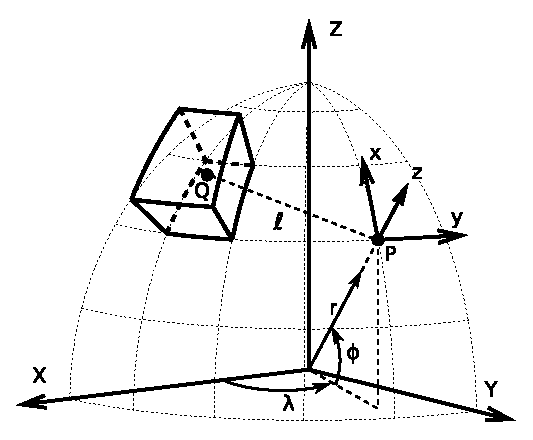
\includegraphics{figs/tesseroid}
    \caption{
        View of a tesseroid,
        the integration point $Q$ inside the tesseroid,
        a geocentric coordinate system $(X, Y, Z)$,
        the computation $P$ and it's local coordinate system $(x, y, z)$.
        $r$, $\phi$, $\lambda$ are
        the radius, latitude, and longitude, respectively, of point $P$,
        and $\ell$ is the Cartesian distance between $P$ and $Q$.
    }
    \label{fig:tesseroid}
\end{figure}

Equations
\ref{eq:tesspot},
\ref{eq:tessgrav},
and
\ref{eq:tesstensor}
must be numerically integrated
\citep{Grombein2013}.
We follow \citet{Asgharzadeh2007}
and use the 3D Gauss-Legendre Quadrature (GLQ) integration.
The GLQ
approximates the integral by
a weighted sum
\citep{Hildebrand1987},
e.g.

\begin{equation}
    \int\limits_a^b f(x) dx \approx
    \frac{b-a}{2}\sum\limits_{i=1}^N W_i f(x_i),
\end{equation}

\noindent
where
$W_i$ are weights and
the discretization points (nodes) $x_i$
are the roots of the $N$th order Legendre polynomial $P_N$.
Note that the roots have to be scaled to the integration limits.
The roots of a second-order Legendre polynomial are
$x_1=-0.577350269$ and $x_2=0.577350269$.
For an arbitrary order $N$,
we have used the root-finder algorithm
of \citet{Barrera-Figueroa2006}
to calculate the roots of $P_N$.
The weights $W_i$ are \citep{Hildebrand1987}

\begin{equation}
    W_i = \frac{2}{(1 - x_i^2)(P'_N(x_i))^2},
\end{equation}

\noindent
where $P'_N$ is the first derivative of $P_N$.

The triple integrals in equations
\ref{eq:tesspot},
\ref{eq:tessgrav},
and
\ref{eq:tesstensor}
become

\begin{equation}
    V(r,\phi,\lambda) \approx
        A
        \sum\limits_{k=1}^{N^{\lambda}}
        \sum\limits_{j=1}^{N^{\phi}}
        \sum\limits_{i=1}^{N^r}
        W^r_i W^{\phi}_j W^{\lambda}_k
        \frac{1}{\ell} \kappa,
\end{equation}
\begin{equation}
    g_{\alpha}(r,\phi,\lambda) \approx
        A
        \sum\limits_{k=1}^{N^{\lambda}}
        \sum\limits_{j=1}^{N^{\phi}}
        \sum\limits_{i=1}^{N^r}
        W^r_i W^{\phi}_j W^{\lambda}_k
        \frac{\Delta_{\alpha}}{\ell^3} \kappa,
\end{equation}

\noindent
and

\begin{equation}
    g_{\alpha\beta}(r,\phi,\lambda) \approx
        A
        \sum\limits_{k=1}^{N^{\lambda}}
        \sum\limits_{j=1}^{N^{\phi}}
        \sum\limits_{i=1}^{N^r}
        W^r_i W^{\phi}_j W^{\lambda}_k
        I_{\alpha\beta},
\end{equation}

\noindent
where

\begin{equation}
    A = G \rho
    \frac{(\lambda_2 - \lambda_1)(\phi_2 - \phi_1)(r_2 - r_1)}{8},
\end{equation}

\noindent
$W_i^r$, $W_j^{\phi}$, and $W_k^{\lambda}$
are the weights
and $N^r$, $N^{\phi}$, and $N^{\lambda}$
are the number of nodes
for the radial, latitudinal, and longitudinal dimensions, respectively.

The accuracy of the integration
depends on the number of nodes, or GLQ order,
used in the discretization.
However, \citet{Ku1977} showed
that it also depends on the ratio between
the distance to the computation point
and the distance between adjacent nodes.
Fig.~\ref{fig:sample}
illustrates this effect
on the $g_{xy}$ gravity gradient component.
To increase the accuracy of the integration,
one could increase the number of nodes,
as in Fig.~\ref{fig:sample}c.
Likewise,
one could keep the number of nodes fixed
and instead divide the tesseroid into smaller ones.
This would increase the total number of nodes
and effectively decrease
the distance between adjacent nodes.
The latter is the approach
taken by \citet{Li2011}.
Here, we will follow the same approach
and make some improvements to the algorithm.

\begin{figure*}
    \centering
    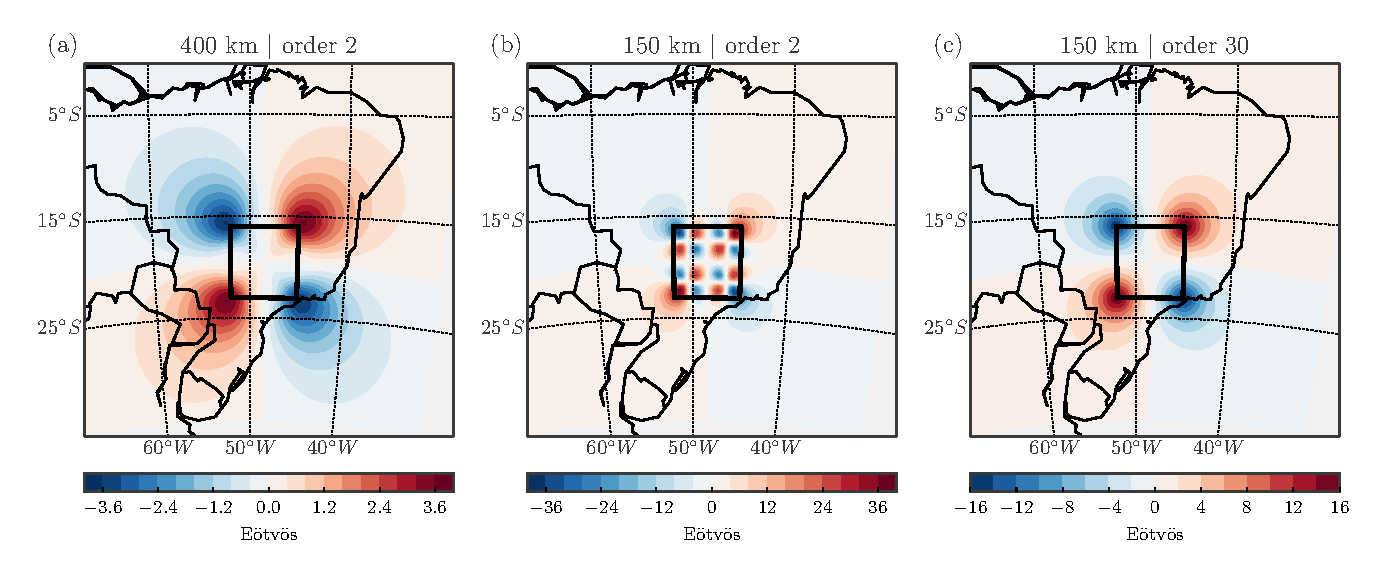
\includegraphics[width=\textwidth]{figs/vary-height-and-order}
    \caption{
        Example of the effect of varying
        the computation height
        and the number of nodes in the Gauss-Legendre Quadrature
        (i.e., the GLQ order).
        The $g_{xy}$ component was produced by a
        $7^\circ \times 7^\circ \times 20\ km$ tesseroid
        with $2.67\ g.cm^{-3}$ density
        and top at $z=0\ km$.
        The maps were calculated on a regular grid
        with $100\times100$ points.
        The GLQ order used was the same
        in the radial, longitudinal, and latitudinal dimensions.
        Black circles represent the horizontal location of the GLQ nodes
        (not shown for GLQ order 30).
        a) Field calculated at $400\ km$ height using GLQ order 2.
        The effect is similar to that presented by \citet{Asgharzadeh2007}.
        b) At $150\ km$ height and order 2,
        the field resembles that of
        four point sources located at the GLQ nodes.
        This effect was shown by \citet{Ku1977}
        for the case of the $g_z$ component of a right rectangular prism.
        c) At $150\ km$ but with a higher GLQ order of 30,
        the field is similar to that expected for a single mass source.
    }
    \label{fig:sample}
\end{figure*}


\subsection{Recursive division algorithm}

We start by fixing the number of GLQ nodes to
$N^\lambda=N^\phi=N^r=2$.
In this way, the distances between adjacent nodes
can be roughly approximated by the dimensions of the tesseroid
(Fig.~\ref{fig:sample}a-b).
Thus, we may use the tesseroid dimensions
as proxies for the distance between nodes.
We define the dimensions of a tesseroid
in the radial, latitudinal, longitudinal directions, respectively,
as

\begin{eqnarray}
    L_r &=& r_2 - r_1,\\
    L_\phi &=& R(\phi_2 - \phi_1),\\
    L_\lambda &=& R(\lambda_2 - \lambda_1),
\end{eqnarray}

\noindent
where $R=6,378,137\ m$ is the mean Earth radius.
The longitudes and latitudes are given in radians.

We write the condition for an accurate GLQ integration
described by \citet{Ku1977}
as a function of
the average of the dimensions of the tesseroid, $L$,

\begin{equation}
    \frac{d}{L} > 1,
\end{equation}

\noindent
where $d$ is the Cartesian distance
between the computation point $P$
and the center of the top face of the tesseroid
(Fig.~\ref{fig:ratio}a).
In a more general form, the condition can be expressed as

\begin{equation}
    \frac{d}{L} > r,
    \label{eq:ratio}
\end{equation}

\noindent
for a positive non-zero scalar $r$,
henceforth referred to as
the ``distance-size ratio''.

To guarantee that equation~\ref{eq:ratio} is satisfied,
one could divide the tesseroid in half for each of the three dimensions.
The division would be repeated recursively
for each of the eight smaller tesseroids
until equation~\ref{eq:ratio} is satisfied for all smaller tesseroids.
Then, the effect of the original tesseroid can be calculated
as the sum of the
effects of the smaller tesseroids,
each of which is calculated using a second-order GLQ.

However, this would result in unnecessary divisions,
specially if one dimension of the tesseroid is much smaller than the others.
A more efficient approach is
to check if equation~\ref{eq:ratio} is met
for each of the three dimensions of the tesseroid
($L_r$, $L_\phi$, and $L_\lambda$).
We only divide the tesseroid in half
along dimensions for which the condition is not met.

This algorithm can be implemented
in the form of a recursive function
as follows:

\begin{verbatim}
function gravity(P, model):
  result = 0
  for each tesseroid in model:
    d = distance from P to the top of tesseroid
    if d/L_lon < r:
      divide_lon = true
    if d/L_lat < r:
      divide_lat = true
    if d/L_r < r:
      divide_r = true
    if divide_lon or divide_lat or divide_r:
      newmodel = (divide tesseroid in the
                  required dimensions)
      result = result + gravity(P, newmodel)
    else
      result = result + effect of tesseroid
  return result
\end{verbatim}

The distance-size ratio $r$ controls
how far away $P$ has to be
compared to the dimensions of the tesseroid.
A ratio $r=2$ means that
the recursive division algorithm will ensure that
tesseroids are smaller than
half the distance to $P$.
Thus, the ratio determines how many divisions are required.
Fig.~\ref{fig:ratio}
illustrates the recursive division of a tesseroid
(Fig.~\ref{fig:ratio}a)
using increasing values of $r$.
The tesseroid is divided into
$28$ tesseroids for $r=1$ (Fig.~\ref{fig:ratio}b),
$146$ tesseroids for $r=2$ (Fig.~\ref{fig:ratio}c),
and $3106$ tesseroids for $r=6$ (Fig.~\ref{fig:ratio}d).

Because the number of tesseroids increases with $r$,
so does the computation time.
Hence, there is need to determine
an optimal value of the distance-size ratio $r$
that yields an acceptable trade-off between
accuracy and computation time.
In the following section,
we describe a methodology
to quantify the error of the GLQ integration
as a function of the distance-size ratio $r$.
These results can be used
to determine optimal values of $r$
for the gravitational potential,
gravitational attraction,
and gravity gradient tensor.

\begin{figure}
    \centering
    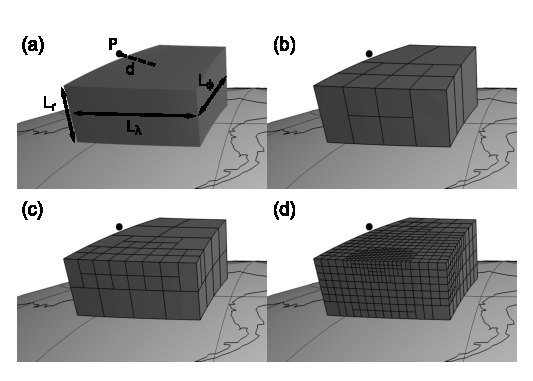
\includegraphics{figs/tesseroid-split}
    \caption{
        Adaptive discretization
        of the tesseroid shown in (a)
        for a computation point P
        using the distance-size ratio $r$ equal to
        (b) 1, (c) 2, and (d) 6.
        $d$ is the Cartesian distance between
        the center of the top face of the tesseroid
        and $P$.
        $L_r$, $L_\phi$, and $L_\lambda$ are the dimensions of the tesseroid.
        Note that increasing $r$
        results in a fine division of the tesseroid
        close the computation point
        and a coarser division further away.
    }
    \label{fig:ratio}
\end{figure}

\subsection{Comparison with a spherical shell}

We must establish reference values
to evaluate the error of the numerical integration.
For this purpose, we have used a homogeneous spherical shell
with its bottom at a sphere with radius $R$ (the mean Earth radius),
thickness $\Delta r$, and density $\rho$.
It is a convenient geometry
with analytical solutions for
the gravitational potential, attraction, and gravity gradient tensor
\citep{Grombein2013}

\begin{equation}
V(r) = \frac{4}{3}\pi G \rho \frac{r_2^3 - r_1^3}{r},
\end{equation}

\begin{equation}
g_z(r) = \frac{V(r)}{r},
\end{equation}

\begin{equation}
g_{zz}(r) = 2\frac{V(r)}{r^2},
\end{equation}

\begin{equation}
g_{xx}(r) = g_{yy}(r) = -\frac{g_{zz}}{2},
\end{equation}

\noindent
and

\begin{equation}
g_x(r) = g_y(r) = g_{xy}(r) = g_{xz}(r) = g_{yz}(r) = 0,
\end{equation}

\noindent
where $r$ is the radial coordinate of the computation point and
$r_1 = R$ and $r_2 = r_1 + \Delta r$ are radial coordinates
of the bottom and top of the spherical shell, respectively.
Table~\ref{tab:shell} summarises the parameters defining the spherical shell.

The computation point can be considered at any longitude or latitude because of
the symmetry of the spherical shell.

The spherical shell had dimensions of $r_1 = R$ ($R$ is the mean Earth radius) and $r_2 = R +
1\ km$ and density $\rho = 2.67\ g.cm^{-3}$.

The largest errors due are concentrated directly on top of the tesseroid
(Fig.~\ref{fig:sample}b).

Therefore, we perform the computations on an $11 \times 11$ point regular grid
in an area directly on top of the tesseroid with corner at $\lambda = 0^\circ$
$\phi = 0^\circ$.


The computation grid was located at a constant height above the spherical shell
$h = r_2 + 1\ km$.



\begin{table}
    \caption{Parameters of the spherical shell.}
    \label{tab:shell}
    \begin{tabular}{lr}
        $\rho$                    & $2.67\ g.cm^{-3}$ \\
        $\Delta r$                & $1\ km$ \\
        $r_1 = R$                 & $6,378.137\ km$ \\
        $r_2 = r_1 + \Delta r$    & $6,379.137\ km$ \\
    \end{tabular}
\end{table}


\subsection{Software implementation}

The recursive division algorithm described above
is implemented in the software package
Tesseroids.
The package consists
of command-line programs
written in the C programming language.
Tesseroids is open-source software
and is freely available
on the internet\footnote{www.leouieda.com/tesseroids}
\textbf{CITE ARCHIVE} provides a persistent
archive for the source code.

The code used to produce the results and figures presented here
is available at \textbf{DOI LINK AND CITATION}.


%%%%%%%%%%%%%%%%%%%%%%%%%%%%%%%%%%%%%%%%%%%%%%%%%%%%%%%%%%%%%%%%%%%%%%%%%%%%%%
\section{Results}

Meh.

\begin{figure*}
    \centering
    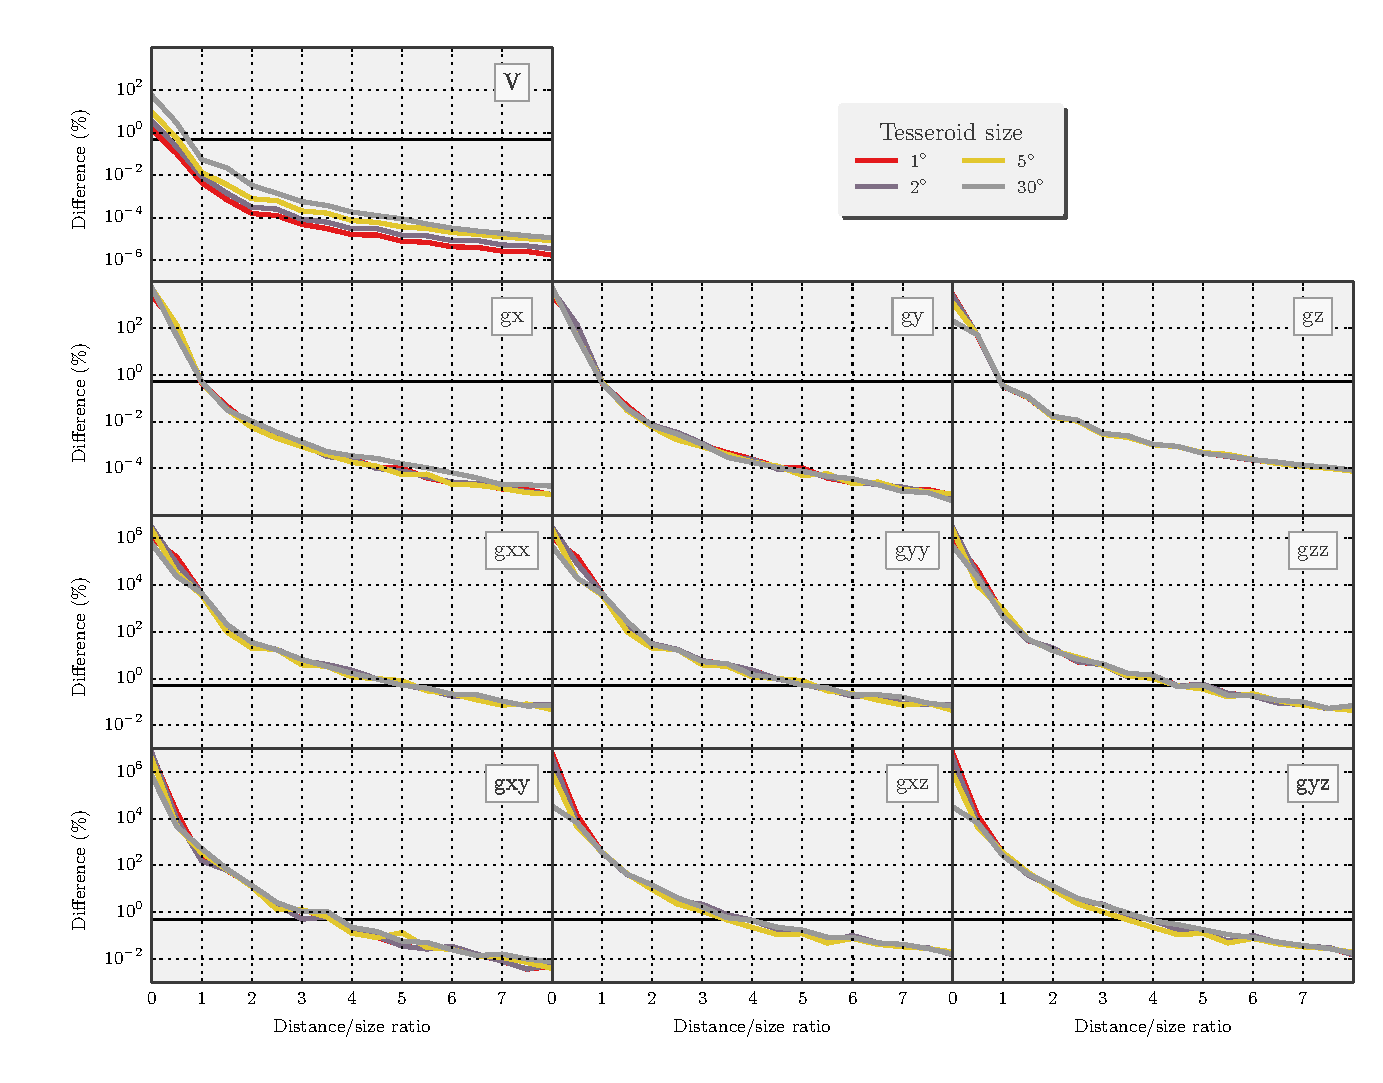
\includegraphics[width=\textwidth]{figs/tesseroid-x-shell}
    \caption{
        Tesseroid vs spherical shell.
    }
    \label{fig:tesseroid-x-shell}
\end{figure*}

%%%%%%%%%%%%%%%%%%%%%%%%%%%%%%%%%%%%%%%%%%%%%%%%%%%%%%%%%%%%%%%%%%%%%%%%%%%%%%
\section{Discussion}

%%%%%%%%%%%%%%%%%%%%%%%%%%%%%%%%%%%%%%%%%%%%%%%%%%%%%%%%%%%%%%%%%%%%%%%%%%%%%%
\section{Conclusions}

%%%%%%%%%%%%%%%%%%%%%%%%%%%%%%%%%%%%%%%%%%%%%%%%%%%%%%%%%%%%%%%%%%%%%%%%%%%%%%
\section{Acknowledgments}
